\documentclass[border=4pt]{standalone}
\usepackage{tikz}
\usetikzlibrary{arrows.meta, calc, decorations.markings}
\usepackage{amsmath}

\definecolor{traitor}{HTML}{b2182b}
\definecolor{faithful}{HTML}{2166ac}
\definecolor{dead}{HTML}{cccccc}
\definecolor{accent}{HTML}{1b7837}
\definecolor{warn}{HTML}{e08214}
\definecolor{panelbg}{HTML}{fafafa}

\begin{document}
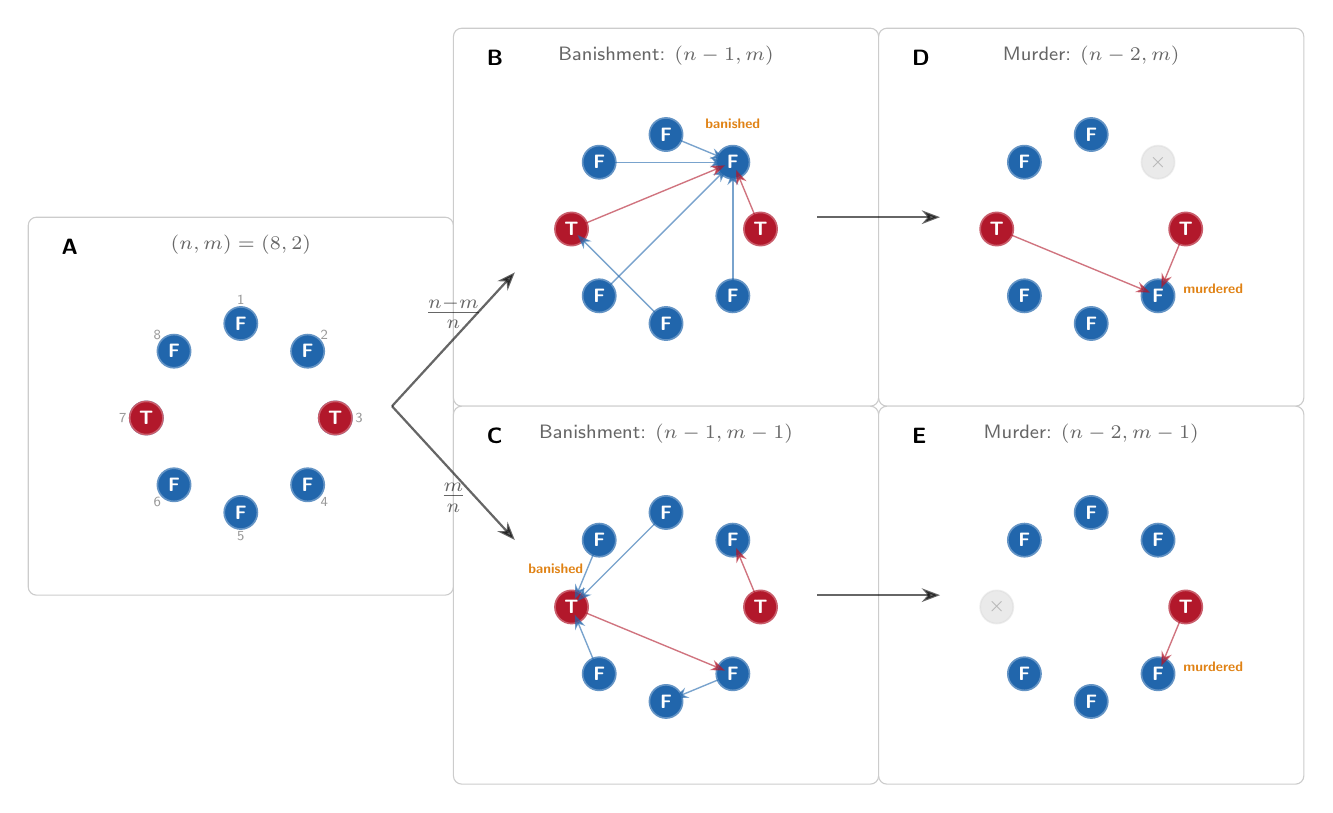
\begin{tikzpicture}[
    >=Stealth,
    font=\sffamily,
    player/.style={circle, minimum size=12pt, inner sep=0pt, line width=0.6pt,
                   font=\sffamily\scriptsize\bfseries, text=white},
    fnode/.style={player, fill=faithful, draw=faithful!70},
    tnode/.style={player, fill=traitor, draw=traitor!70},
    dnode/.style={player, fill=dead, draw=dead!80, opacity=0.4,
                  font=\sffamily\scriptsize\bfseries, text=black!60},
    votearrow/.style={->, line width=0.5pt, opacity=0.6},
    killarrow/.style={->, line width=1.0pt, traitor, opacity=0.8},
    panellabel/.style={font=\sffamily\footnotesize\bfseries, anchor=north west},
    caption/.style={font=\sffamily\scriptsize, text=black!60, align=center},
]

% ── Layout: 2 rows x 3 cols, each panel ~4.2cm wide ──
\def\pw{4.8}   % panel width
\def\ph{4.2}   % panel height
\def\gap{0.6}  % gap between panels
\def\R{1.2}    % circle radius for players

% Panel origins (bottom-left of each)
\coordinate (P1) at (0, \ph-3*\gap);
\coordinate (P2) at (\pw+\gap, \ph+\gap);
\coordinate (P3) at (2*\pw+2*\gap, \ph+\gap);
\coordinate (P5) at (\pw+\gap, 0);
\coordinate (P6) at (2*\pw+2*\gap, 0);

% ── Helper: draw 8 players in a circle ──
% Args: center, prefix, traitor list (1-indexed)
\newcommand{\drawplayers}[3]{
    % #1 = center, #2 = prefix, #3 = comma-separated traitor positions
    \foreach \i in {1,...,8} {
        \pgfmathsetmacro{\angle}{90 - (\i-1)*45}
        \coordinate (#2-\i) at ($(#1) + (\angle:\R)$);
    }
    % Draw faithful first (F label), then traitors on top (T label)
    \foreach \i in {1,...,8} {
        \node[fnode] at (#2-\i) {F};
    }
    \foreach \t in {#3} {
        \node[tnode] at (#2-\t) {T};
    }
}

% ══════════════════════════════════════════════════════════════
% TOP ROW: Game phases
% ══════════════════════════════════════════════════════════════

% ── Panel A: Roles ──
\begin{scope}[shift=(P1)]
    \draw[draw=black!20, fill=white, rounded corners=3pt] (-0.3, -0.3) rectangle (\pw+0.3, \ph+0.3);
    \node[panellabel] at (0, \ph+0.15) {A};
    \node[caption] at (\pw/2, \ph-0.05) {\((n, m)=(8, 2)\)};

    \pgfmathsetmacro{\cx}{\pw/2}
    \pgfmathsetmacro{\cy}{\ph/2 - 0.15}
    \coordinate (CA) at (\cx, \cy);
    \drawplayers{CA}{a}{3,7}

    % % Legend
    % \node[fnode, minimum size=10pt] at (3.35, 0.6) {F};
    % \node[font=\sffamily\tiny, text=faithful, anchor=west] at (3.55, 0.6) {Faithful};
    % \node[tnode, minimum size=10pt] at (3.35, 0.25) {T};
    % \node[font=\sffamily\tiny, text=traitor, anchor=west] at (3.55, 0.25) {Traitor};

    % Player numbers
    \foreach \i in {1,...,8} {
        \pgfmathsetmacro{\angle}{90 - (\i-1)*45}
        \node[font=\sffamily\tiny, text=black!40] at ($(CA) + (\angle:\R+0.3)$) {\i};
    }
\end{scope}

% ── Panel B: Night (Murder) ──
\begin{scope}[shift=(P2)]
    \draw[draw=black!20, fill=white, rounded corners=3pt] (-0.3, -0.3) rectangle (\pw+0.3, \ph+0.3);
    \node[panellabel] at (0, \ph+0.15) {B};
    \node[caption] at (\pw/2, \ph-0.05) {Banishment: \((n - 1, m)\)};

    \pgfmathsetmacro{\cx}{\pw/2}
    \pgfmathsetmacro{\cy}{\ph/2 - 0.15}
    \coordinate (CC) at (\cx, \cy);

    \foreach \i in {1,...,8} {
        \pgfmathsetmacro{\angle}{90 - (\i-1)*45}
        \coordinate (c-\i) at ($(CC) + (\angle:\R)$);
    }
    \foreach \i in {1,2,4,5,6,8} {
        \node[fnode] at (c-\i) {F};
    }
    \node[tnode] at (c-3) {T};
    \node[tnode] at (c-7) {T};

    \foreach \src in {1,4,6,8} {
        \draw[votearrow, faithful, shorten >=3pt, shorten <=3pt] (c-\src) -- (c-2);
    }
        \draw[votearrow, faithful, shorten >=3pt, shorten <=3pt] (c-5) -- (c-7);
    \draw[votearrow, traitor, shorten >=3pt, shorten <=3pt] (c-3) -- (c-2);
    \draw[votearrow, traitor, shorten >=3pt, shorten <=3pt] (c-7) -- (c-2);

    % Banished marker
    \node[font=\sffamily\tiny\bfseries, text=warn, anchor=south] at ($(c-2)+(0, 0.3)$) {banished};
\end{scope}

% ── Panel C: Day (Banishment) ──
\begin{scope}[shift=(P3)]
    \draw[draw=black!20, fill=white, rounded corners=3pt] (-0.3, -0.3) rectangle (\pw+0.3, \ph+0.3);
    \node[panellabel] at (0, \ph+0.15) {D};
    \node[caption] at (\pw/2, \ph-0.05) {Murder: \((n - 2, m)\)};

    \pgfmathsetmacro{\cx}{\pw/2}
    \pgfmathsetmacro{\cy}{\ph/2 - 0.15}
    \coordinate (CC) at (\cx, \cy);

    \foreach \i in {1,...,8} {
        \pgfmathsetmacro{\angle}{90 - (\i-1)*45}
        \coordinate (c-\i) at ($(CC) + (\angle:\R)$);
    }
    \foreach \i in {1,4,5,6,8} {
        \node[fnode] at (c-\i) {F};
    }
    \node[tnode] at (c-3) {T};
    \node[tnode] at (c-7) {T};
    \node[dnode] at (c-2) {$\times$};

    % Show some votes converging on player 2 (banished)
    \draw[votearrow, traitor, shorten >=3pt, shorten <=3pt] (c-3) -- (c-4);
    \draw[votearrow, traitor, shorten >=3pt, shorten <=3pt] (c-7) -- (c-4);

    % Banished marker
    \node[font=\sffamily\tiny\bfseries, text=warn, anchor=south] at ($(c-4)+(.7, -.1)$) {murdered};
\end{scope}

\begin{scope}[shift=(P5)]
    \draw[draw=black!20, fill=white, rounded corners=3pt] (-0.3, -0.3) rectangle (\pw+0.3, \ph+0.3);
    \node[panellabel] at (0, \ph+0.15) {C};
    \node[caption] at (\pw/2, \ph-0.05) {Banishment: \((n - 1, m - 1)\)};

    \pgfmathsetmacro{\cx}{\pw/2}
    \pgfmathsetmacro{\cy}{\ph/2 - 0.15}
    \coordinate (CC) at (\cx, \cy);

    \foreach \i in {1,...,8} {
        \pgfmathsetmacro{\angle}{90 - (\i-1)*45}
        \coordinate (c-\i) at ($(CC) + (\angle:\R)$);
    }
    \foreach \i in {1,2,4,5,6,8} {
        \node[fnode] at (c-\i) {F};
    }
    \node[tnode] at (c-3) {T};
    \node[tnode] at (c-7) {T};

    % Show some votes converging on player 2 (banished)
    \foreach \src in {1,6,8} {
        \draw[votearrow, faithful, shorten >=3pt, shorten <=3pt] (c-\src) --
        (c-7);
    }
    \draw[votearrow, faithful, shorten >=3pt, shorten <=3pt] (c-4) -- (c-5);
    \draw[votearrow, traitor, shorten >=3pt, shorten <=3pt] (c-3) -- (c-2);
    \draw[votearrow, traitor, shorten >=3pt, shorten <=3pt] (c-7) -- (c-4);

    % Banished marker
    \node[font=\sffamily\tiny\bfseries, text=warn, anchor=south] at ($(c-7)+(-.2, 0.3)$) {banished};
\end{scope}

\begin{scope}[shift=(P6)]
    \draw[draw=black!20, fill=white, rounded corners=3pt] (-0.3, -0.3) rectangle (\pw+0.3, \ph+0.3);
    \node[panellabel] at (0, \ph+0.15) {E};
    \node[caption] at (\pw/2, \ph-0.05) {Murder: \((n - 2, m - 1)\)};

    \pgfmathsetmacro{\cx}{\pw/2}
    \pgfmathsetmacro{\cy}{\ph/2 - 0.15}
    \coordinate (CC) at (\cx, \cy);

    \foreach \i in {1,...,8} {
        \pgfmathsetmacro{\angle}{90 - (\i-1)*45}
        \coordinate (c-\i) at ($(CC) + (\angle:\R)$);
    }
    \foreach \i in {1,2,4,5,6,8} {
        \node[fnode] at (c-\i) {F};
    }
    \node[tnode] at (c-3) {T};
    \node[dnode] at (c-7) {$\times$};

    % Show some votes converging on player 2 (banished)
    \draw[votearrow, traitor, shorten >=3pt, shorten <=3pt] (c-3) -- (c-4);

    % Banished marker
    \node[font=\sffamily\tiny\bfseries, text=warn, anchor=south] at ($(c-4)+(.7, -.1)$) {murdered};
\end{scope}

\draw[->, line width=0.8pt, opacity=0.6] (P1) + (\pw*.9, \ph/2) -- ($(P2) + (\pw/10, \ph/3)$)
    node[midway, above] {\(\frac{n - m}{n}\)};
\draw[->, line width=0.8pt, opacity=0.6] (P1) + (\pw*.9, \ph/2) -- ($(P5) + (\pw/10, 2*\ph/3)$)
    node[midway, below] {\(\frac{m}{n}\)};
\draw[->, line width=0.8pt, opacity=0.6] (P2) + (\pw*.9, \ph/2) -- ($(P3) + (\pw/10, \ph/2)$)
    node[midway, below] {};
\draw[->, line width=0.8pt, opacity=0.6] (P5) + (\pw*.9, \ph/2) -- ($(P6) + (\pw/10, \ph/2)$)
    node[midway, below] {};

\end{tikzpicture}
\end{document}
